\documentclass[11pt]{article}
\usepackage[utf8]{inputenc}
\usepackage[T1]{fontenc}
\usepackage{lmodern}
\usepackage[letterpaper,margin=2cm]{geometry}
\usepackage{graphicx}
\usepackage{float}
\usepackage{placeins}
\usepackage{booktabs}
\usepackage{longtable}
\usepackage{array}
\usepackage{amssymb}
\usepackage{amsmath}
\usepackage[font=small]{caption}
\usepackage{microtype}
\usepackage{setspace}
\usepackage{needspace}
\usepackage[hidelinks]{hyperref}
\graphicspath{{figures/}}
\setlength{\parskip}{0.55em}
\setlength{\parindent}{0pt}
\title{"Like, Literally, Love": A Lexical Analysis of Vocabulary Complexity in \emph{Love Island USA} Season 4}
\author{Jeremy Lee}
\date{June 2026}
\begin{document}
\maketitle
\begin{abstract}

This paper asks a simple question about a popular reality show: \emph{how hard is its language?} Using the subtitle transcripts of all 38 episodes of \emph{Love Island USA} Season 4 (2022) --- a 224,815-word corpus of on-screen speech --- we measure vocabulary richness, word frequency, reading level, and the size of vocabulary a viewer actually needs. The answer is consistent across every measure: the show's language is small, repetitive, and very easy. The 100 most common words make up 61\% of everything said, and word frequency follows Zipf's Law almost perfectly (R\textsuperscript{2} = 0.98). A viewer who knows only the \textbf{$\sim$1,250 most common word families understands 95\% of the show} --- less than half the $\sim$3,000 word families normally needed for everyday English. By standard formulas the dialogue reads at roughly a \textbf{3rd--5th grade level}, and 98\% of all words spoken come from the 3,000 most familiar words in English. The talk is emotional and opinion-heavy but lexically thin: adjectives make up only 8.4\% of words, and a handful of discourse markers (\emph{like}, \emph{know}, \emph{yeah}) do much of the work. The show presents its audience with a narrow, highly accessible slice of English.

\end{abstract}
\smallskip\noindent\textbf{Keywords:} lexical diversity, reality television, vocabulary load, readability, corpus linguistics, \emph{Love Island}


\section*{Key Findings at a Glance}

\begin{itemize}
\item \textbf{You need very few words to follow it.} Knowing the $\sim$1,250 most frequent word families is enough to understand 95\% of all speech in the show; $\sim$2,550 gets you to 98\%. For comparison, understanding everyday English normally takes about 3,000 word families for 95\% coverage and 6,000--7,000 for 98\%.
\item \textbf{It reads at roughly a 3rd--5th grade level.} Flesch--Kincaid puts the dialogue at grade 2.8 and a reading-ease score of 90/100 ("very easy"). 97.9\% of all words spoken are among the 3,000 most familiar English words --- so the general public would have no trouble understanding it.
\item \textbf{A tiny core of words dominates.} The top 10 words are 22.7\% of all speech; the top 100 are 61\%. Word frequencies follow Zipf's Law almost exactly (R\textsuperscript{2} = 0.98).
\item \textbf{Low lexical diversity.} Mean MTLD is 59.96, below the $\sim$72 benchmark for ordinary spontaneous speech, and it does not change across the season.
\item \textbf{Emotional but plain.} Speech is uniformly positive and highly subjective, yet adjectives are only 8.4\% of words; meaning is carried by verbs and pronouns, not rich description.
\end{itemize}


\section*{1. Introduction}

Reality television is one of the dominant media formats of the twenty-first century, and \emph{Love Island} --- a British format now franchised worldwide --- is among the most-watched. Unlike scripted drama, it captures speech roughly as it happens: contestants live in a villa, are filmed continuously, and produce hours of unrehearsed conversation per episode. That makes it a useful, if unusual, window onto a particular register of casual spoken English.

The motivation is a well-known fact from applied linguistics. English has around 170,000 words in current use, an educated adult actively uses perhaps 20,000--35,000, and comfortable everyday conversation needs only about 3,000 high-frequency word families (Nation, 2001; Adolphs \& Schmitt, 2003). If ordinary conversation already concentrates on so few words, informal television may narrow the range even further. This paper measures exactly how narrow.

\textbf{Research questions.}

\begin{enumerate}
\item How concentrated is word usage in \emph{Love Island USA} Season 4, and how lexically diverse is the language overall?
\item How many words must a viewer know to follow the show, and how does that compare with the $\sim$3,000-word benchmark for everyday English?
\item What reading/grade level is the dialogue, relative to the $\sim$grade-5 standard used for materials aimed at the general public?
\item What kinds of words dominate (parts of speech, filler words), and what is the emotional tone across the season?
\end{enumerate}


\section*{2. Background}

\textbf{Measuring vocabulary diversity.} The simplest measure, the Type--Token Ratio (TTR) --- unique words divided by total words --- is intuitive but drops automatically as a text gets longer (Richards, 1987). Length-robust measures are preferred: Root TTR partly corrects for length, and the Measure of Textual Lexical Diversity (MTLD; McCarthy \& Jarvis, 2010) tracks how long a stretch of text can run before its running TTR falls below a threshold. As a rule of thumb, spontaneous speech scores roughly 60--100 on MTLD.

\textbf{How many words you need.} Vocabulary researchers express difficulty as \emph{coverage}: the share of a text you understand if you know its most frequent words. Knowing about 3,000 word families gives roughly 95\% coverage of everyday spoken English, and 6,000--7,000 families gives about 98\% (Adolphs \& Schmitt, 2003; Nation, 2006). Television sits in the same range: Webb and Rodgers (2009) found that $\sim$3,000 families cover 95\% of TV dialogue and $\sim$7,000 cover 98\%. These figures give us a yardstick to compare \emph{Love Island} against.

\textbf{Reading level.} Readability formulas convert sentence length and word length/syllables into a U.S. school grade. Flesch--Kincaid (Kincaid et al., 1975) and the Dale--Chall familiar-word approach (Dale \& Chall, 1948) are standard. Public-facing materials --- surveys, health information, news --- are typically written at a 5th--8th grade level so the general population can follow them, with grade 5 often cited as a conservative target.

\textbf{Reality TV talk.} Prior work finds reality contestants mix private conversation with performance, since they know they are filmed, which can push speech toward safe, broadly understood language (Thornborrow \& Morris, 2004), and toward hedges and vague "approximators" such as \emph{like} and \emph{kind of} (Channell, 1994; Fleiss, 2018). No published study has examined \emph{Love Island USA} specifically; this paper begins to fill that gap.


\section*{3. Methods}

\textbf{Data.} Transcripts of all 38 Season 4 episodes (aired July--August 2022 on Peacock) were scraped from Subslikescript.com and stored as a CSV. After cleaning, the corpus is 224,815 word tokens.

\textbf{Scope.} The source is closed-caption subtitle text with no speaker labels, so it mixes contestant dialogue (the large majority) with host/narrator voiceover and occasional on-screen lyrics. Because the voices cannot be separated automatically, results describe \emph{Love Island USA} speech as broadcast, not any one contestant. This is revisited in Limitations.

\textbf{Processing.} Text was lowercased, stripped of subtitle dashes, metadata, and non-letters (apostrophes kept), and tokenised with NLTK; single-character tokens (\emph{I}, \emph{a}) were removed. Sentence counts use the raw text, before punctuation was stripped.

\textbf{Measures.} Word frequency and cumulative top-\emph{N} coverage; Zipf's Law via regression of log frequency on log rank; lexical diversity (TTR, Root TTR, MTLD per episode); part-of-speech tags (NLTK); sentiment (TextBlob). For the two new questions: \textbf{vocabulary load} was computed by lemmatising tokens to approximate word families and finding how many families are needed for 80/90/95/98\% coverage; \textbf{reading level} was computed with \texttt{textstat} (Flesch--Kincaid grade, Flesch Reading Ease, SMOG, and the Dale--Chall familiar-word list). Analyses use Python 3.12 (\texttt{nltk}, \texttt{textblob}, \texttt{textstat}, \texttt{scipy}, \texttt{pandas}, \texttt{matplotlib}).


\section*{4. Results}

\subsection*{4.1 A small, repetitive core vocabulary}

The corpus contains 224,815 word tokens but only 7,856 distinct word types (about 5,900 word families). Usage is heavily concentrated on a few words. The ten most frequent tokens are \emph{you, to, like, the, and, it, that, know, yeah,} and \emph{do} (Figure 1).

\begin{figure}[H]
\centering
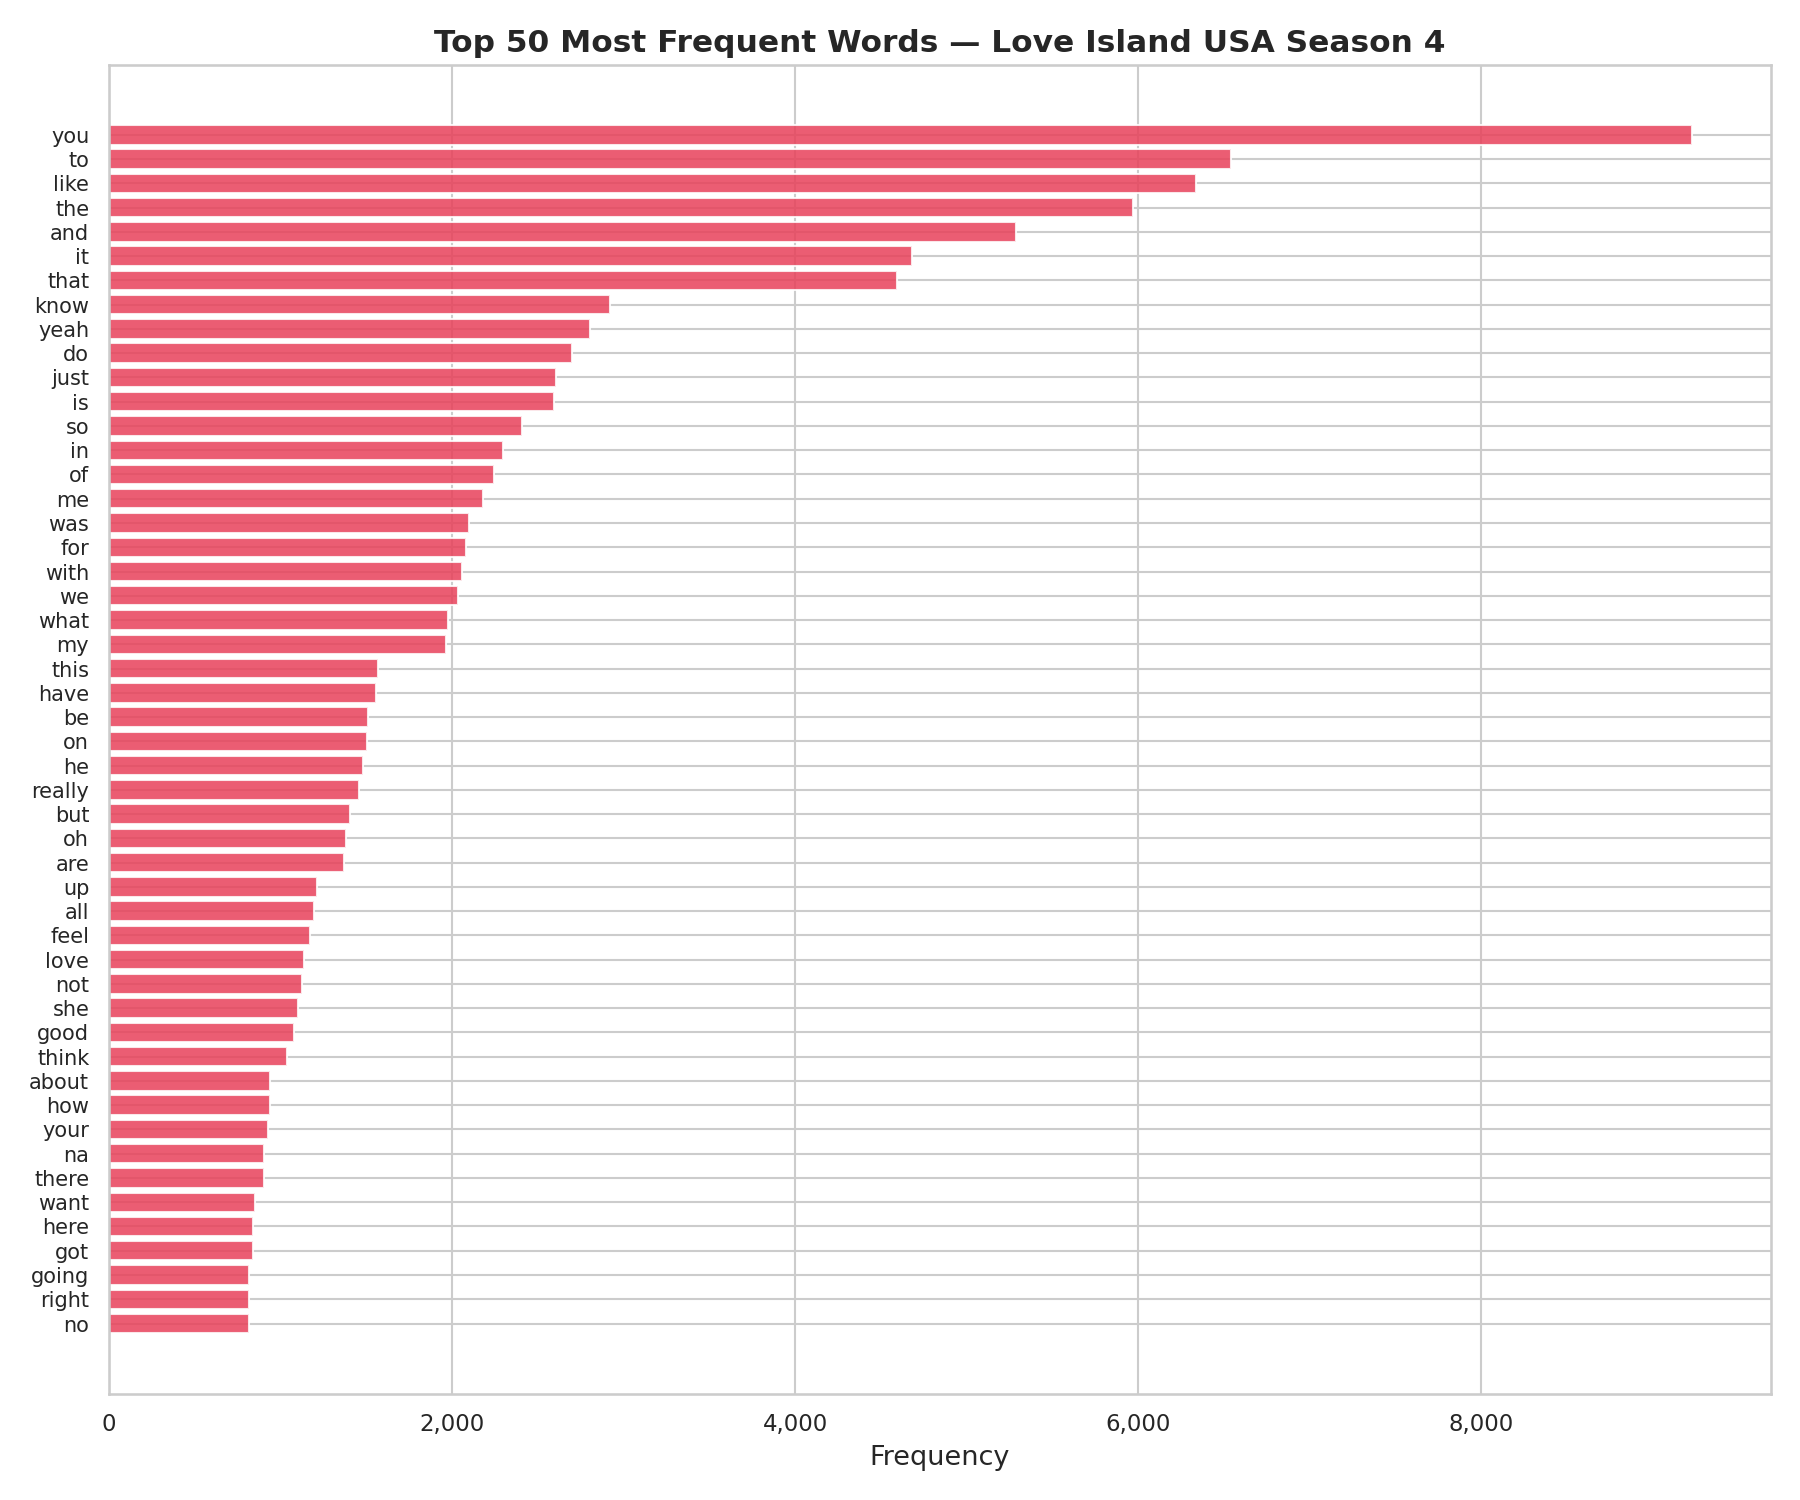
\includegraphics[width=0.82\linewidth,height=0.42\textheight,keepaspectratio]{01_top50_words.png}
\caption*{\textbf{Figure 1.} Top 50 most frequent words.}
\end{figure}

The top 10 words alone are 22.7\% of all speech, the top 50 are 48.7\%, and the top 100 are 61.0\%; a mere 1,000 word types cover 91.1\% of everything said. This is a textbook Zipf distribution: regressing log-frequency on log-rank gives a slope of $-$1.45 with R\textsuperscript{2} = 0.98 (Figure 2). In plain terms, a small number of words are repeated constantly while the long tail of rarer words barely appears.

\begin{figure}[H]
\centering
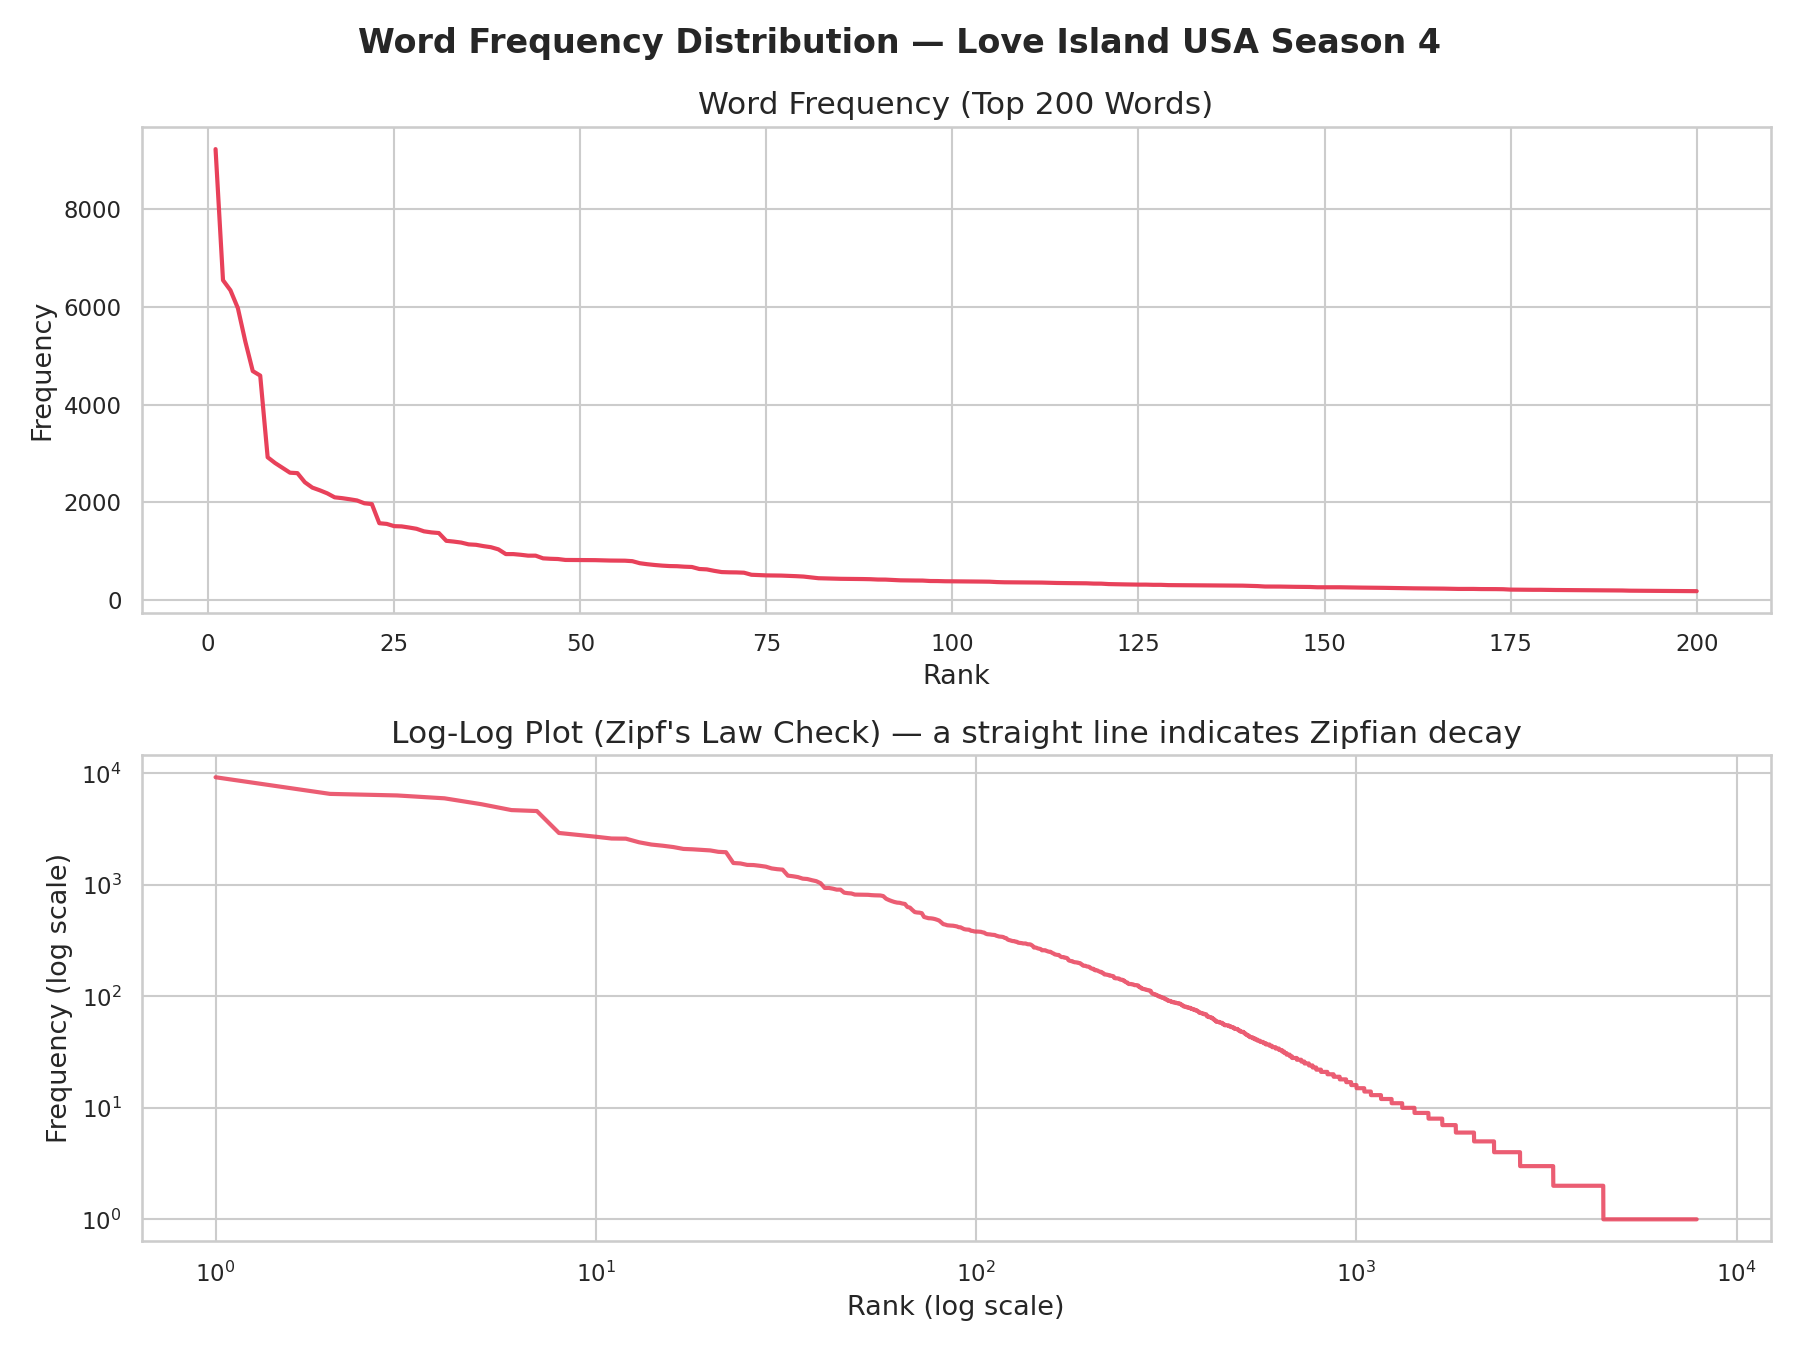
\includegraphics[width=0.82\linewidth,height=0.42\textheight,keepaspectratio]{02_word_frequency_distribution.png}
\caption*{\textbf{Figure 2.} Word frequency distribution and Zipf's Law check.}
\end{figure}

\subsection*{4.2 How many words do you actually need? (RQ2)}

Figure 3 turns frequency into a practical question: if you learned the show's most common words first, how much would you understand? The curve rises steeply and then flattens. Knowing just the \textbf{250 most common word families covers 80\%} of all speech, \textbf{$\sim$590 covers 90\%}, \textbf{$\sim$1,250 covers 95\%}, and \textbf{$\sim$2,550 covers 98\%}.

\begin{figure}[H]
\centering
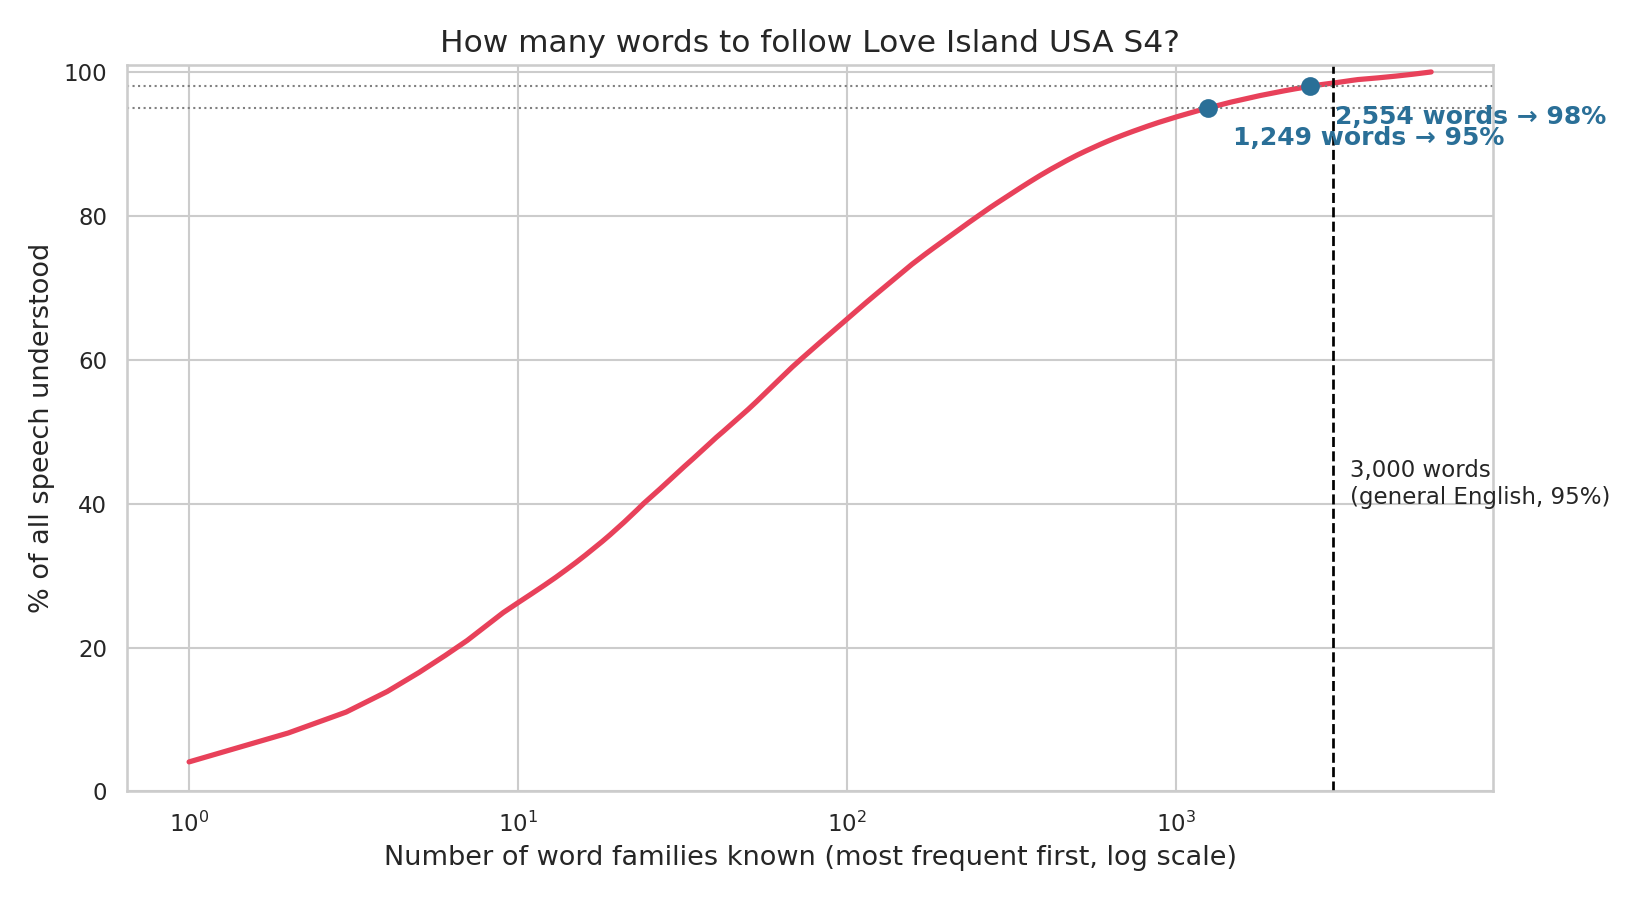
\includegraphics[width=0.82\linewidth,height=0.42\textheight,keepaspectratio]{11_vocabulary_coverage.png}
\caption*{\textbf{Figure 3.} How many words you need to follow the show.}
\end{figure}

Set against the benchmarks, the show is markedly easier than general English. Everyday spoken English needs roughly 3,000 word families for 95\% coverage and 6,000--7,000 for 98\% (Adolphs \& Schmitt, 2003; Nation, 2006; Webb \& Rodgers, 2009). \emph{Love Island} reaches 95\% with \textbf{fewer than half} that vocabulary ($\sim$1,250), and even 98\% of the show ($\sim$2,550 families) falls \emph{below} the 3,000-word everyday-English threshold. A learner or younger viewer with a modest vocabulary could follow almost all of it.

\subsection*{4.3 What reading level is the show? (RQ3)}

By standard readability formulas the dialogue is very easy (Figure 4). Flesch--Kincaid places it at \textbf{grade 2.8} (per-episode range 2.3--3.7), the consensus grade estimate is \textbf{3.0}, and the Flesch Reading Ease score is \textbf{90.2 out of 100} --- the "very easy" band, understandable by an average 11-year-old. Syllable-weighted formulas read slightly higher (SMOG $\approx$ 6.9), because the show does use the occasional long word (\emph{relationship}, \emph{definitely}), but every measure keeps the language at or near the grade-5 mark used for general-public materials --- never in the difficult range.

\begin{figure}[H]
\centering
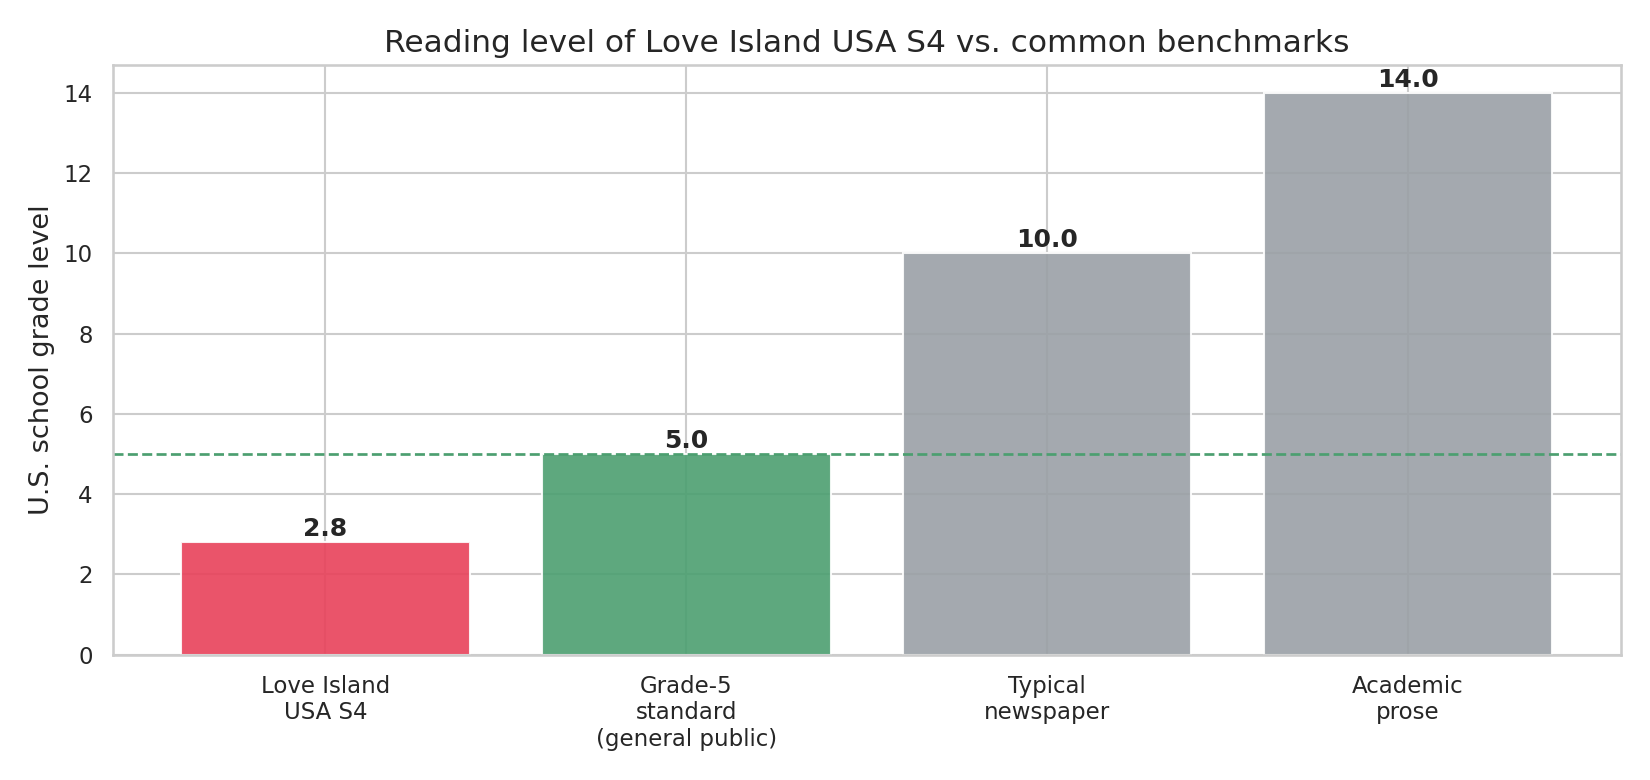
\includegraphics[width=0.82\linewidth,height=0.42\textheight,keepaspectratio]{12_reading_level.png}
\caption*{\textbf{Figure 4.} Reading level (Flesch--Kincaid grade) vs. common benchmarks; other formulas place the show similarly low.}
\end{figure}

The vocabulary evidence agrees: only \textbf{2.1\% of all words spoken fall outside the 3,000 most familiar English words} (the Dale--Chall list known to fourth-graders). Put the other way, 97.9\% of the show's words are among the most familiar in the language. Whether judged by sentence complexity or by word familiarity, \emph{Love Island} is comfortably within reach of the general public.

\subsection*{4.4 Lexical diversity across the season}

Per-episode MTLD averages 59.96 (range 40.42--81.93), below the $\sim$72 benchmark for ordinary spontaneous speech --- i.e., the show is \emph{less} varied than normal conversation. Diversity does not drift over the season: neither MTLD nor TTR correlates with episode number (MTLD: r = $-$0.11, p = .52; TTR: r = 0.05, p = .78). Episode-to-episode bumps in Figure 5 track episode length and content (recaps, finales), not a trend.

\begin{figure}[H]
\centering
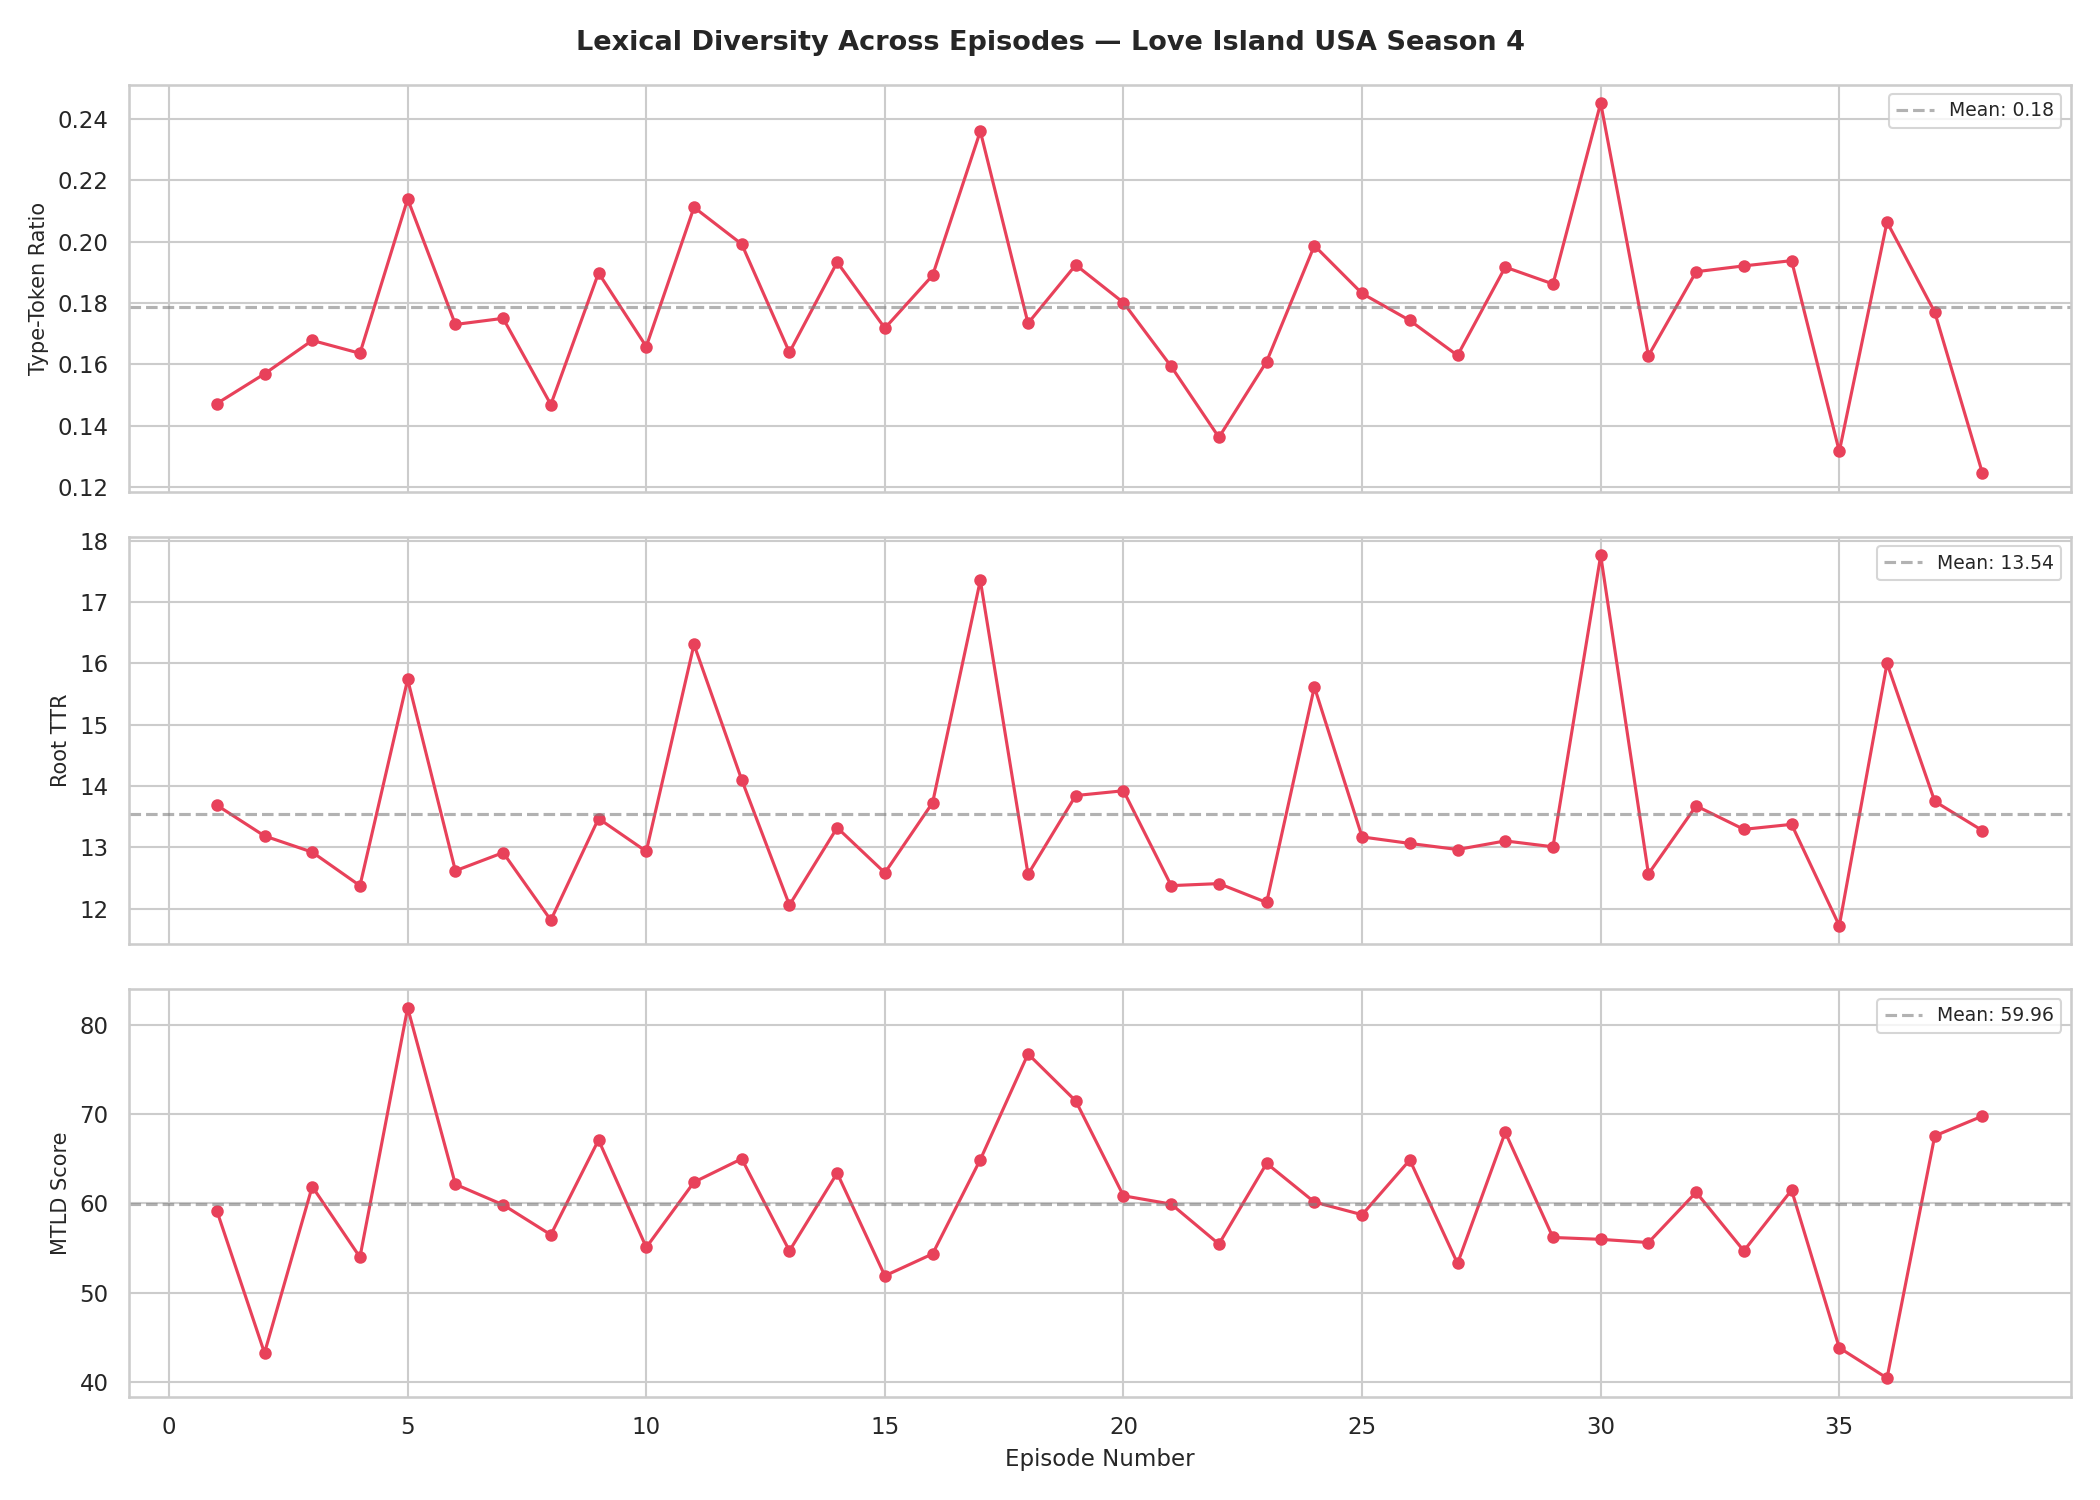
\includegraphics[width=0.82\linewidth,height=0.42\textheight,keepaspectratio]{03_lexical_diversity_per_episode.png}
\caption*{\textbf{Figure 5.} Lexical diversity across episodes.}
\end{figure}

\subsection*{4.5 Filler and hedge words}

Filler and hedge words are pervasive (Figure 6). The most common are \emph{like} (28.2 per 1,000 words), \emph{know} (13.0), and \emph{yeah} (12.5). \emph{Like} alone is more than twice as frequent as any other filler and is the third most common word in the entire corpus. Across the 24 tracked filler/hedge words, these account for 9.3\% of all tokens --- roughly one word in eleven --- doing social and discourse-organising work rather than conveying new information.

\begin{figure}[H]
\centering
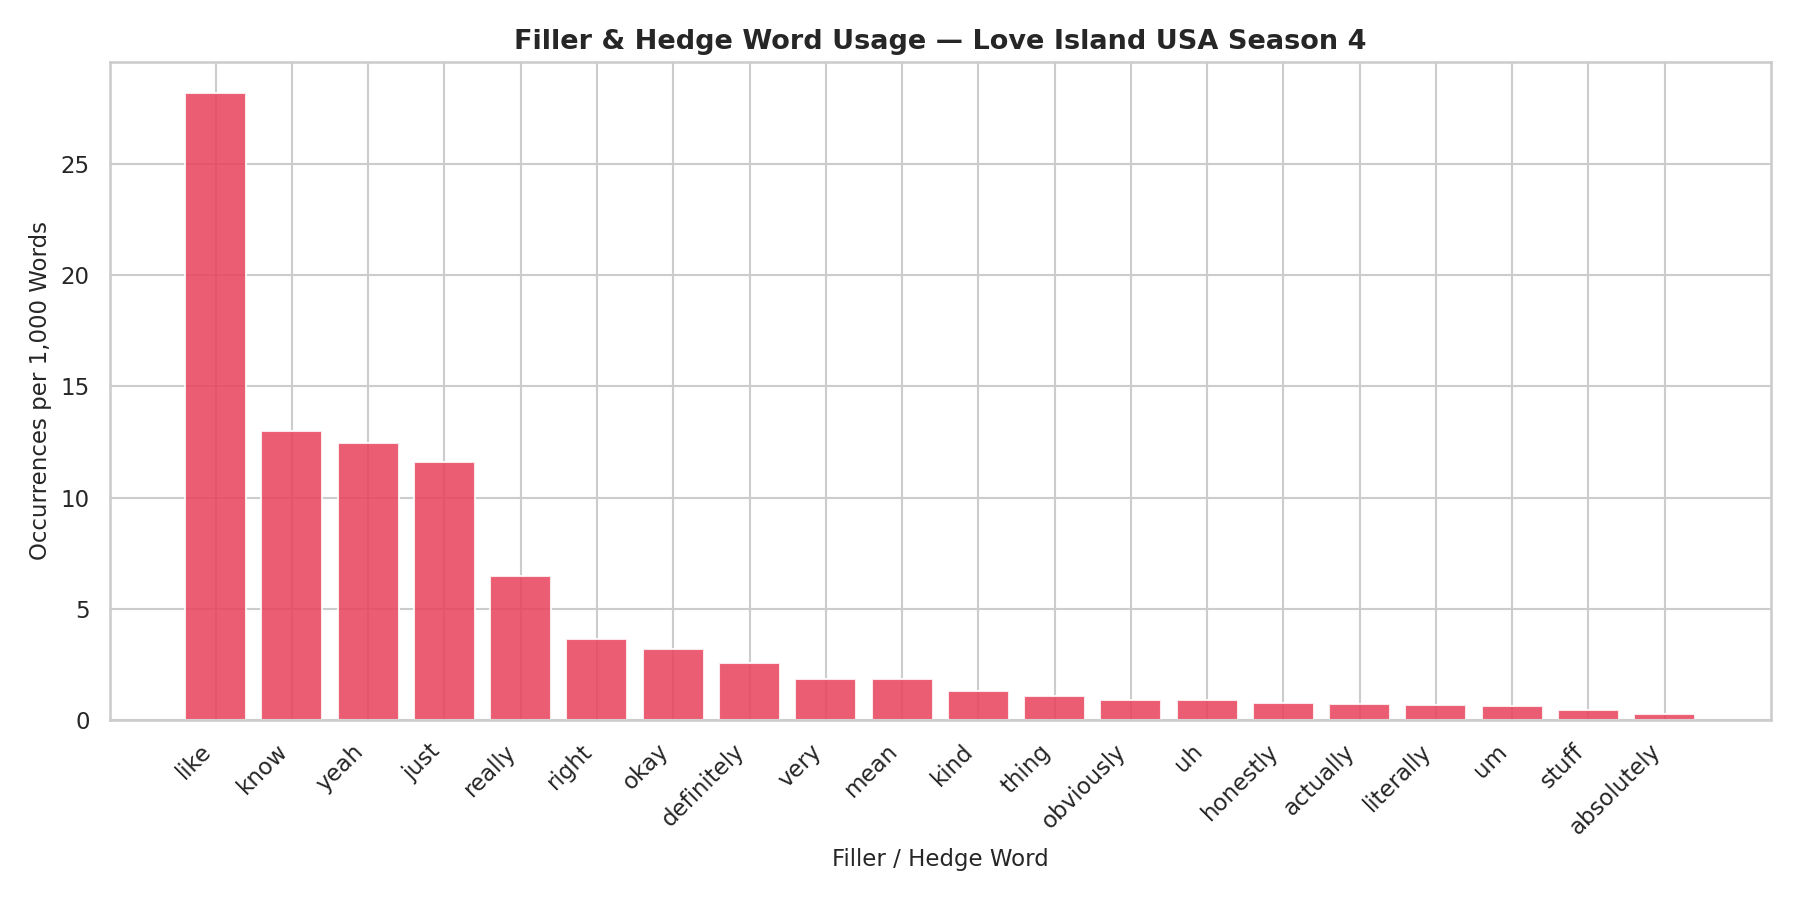
\includegraphics[width=0.82\linewidth,height=0.42\textheight,keepaspectratio]{06_filler_words.png}
\caption*{\textbf{Figure 6.} Filler and hedge word usage.}
\end{figure}

\subsection*{4.6 What kinds of words: parts of speech}

Verbs are the largest word class (24.5\%), then nouns (17.9\%), prepositions (15.4\%), and pronouns (13.6\%). Crucially, \textbf{adjectives are only 8.4\%} of words (adverbs another 8.5\%). Adjectives are the main carriers of description, so their scarcity --- combined with heavy pronoun and verb use --- marks a discourse built on relationships and actions ("I want to", "you said", "we talked") rather than vivid description.

\begin{figure}[H]
\centering
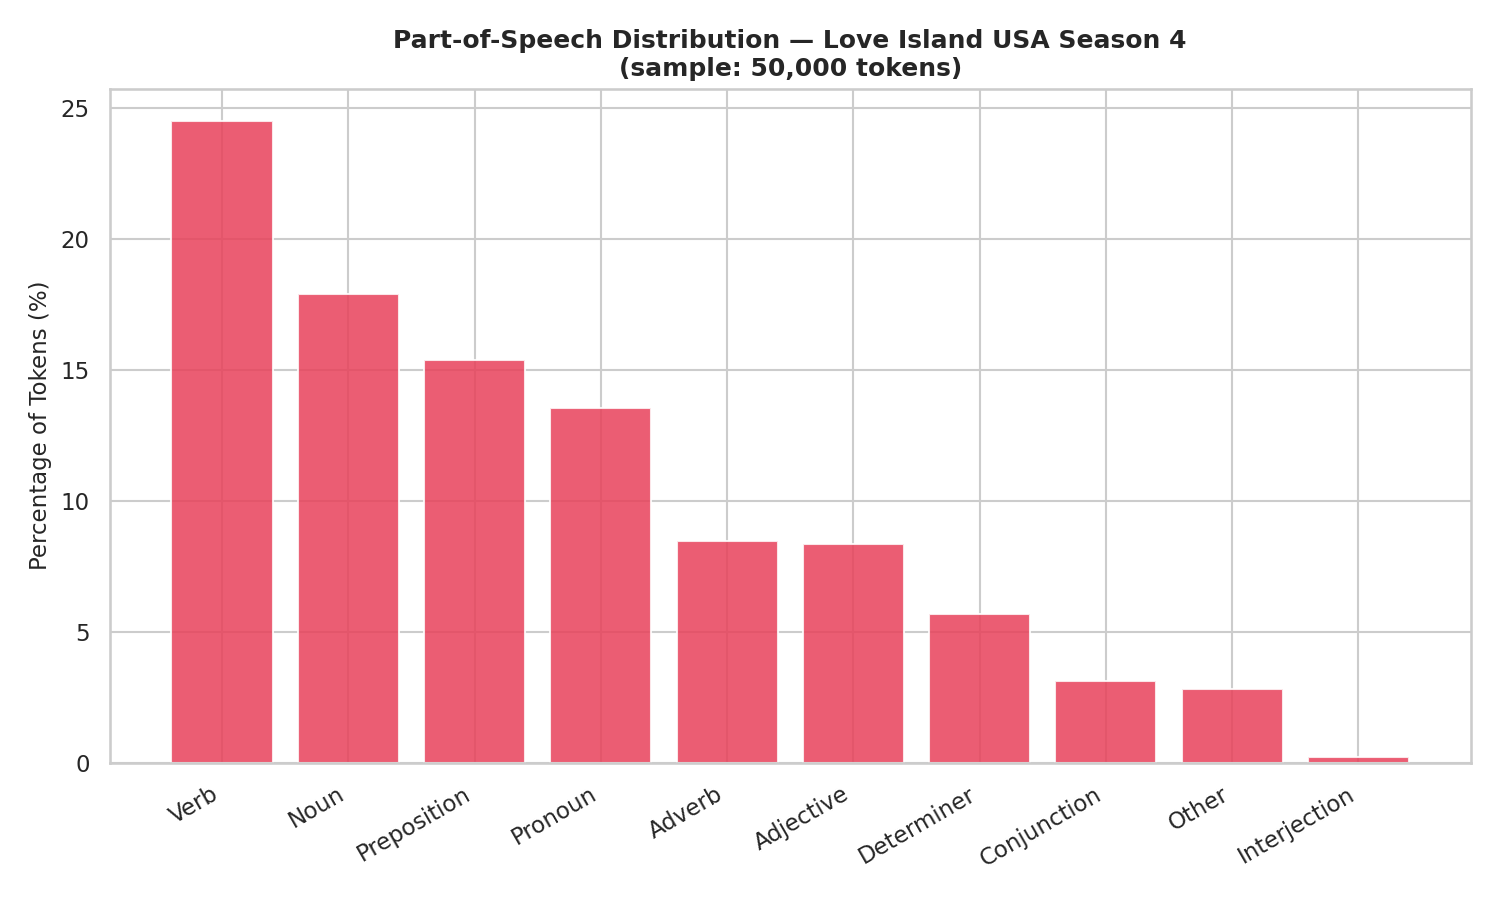
\includegraphics[width=0.82\linewidth,height=0.42\textheight,keepaspectratio]{07_pos_distribution.png}
\caption*{\textbf{Figure 7.} Part-of-speech distribution.}
\end{figure}

\subsection*{4.7 Emotional tone}

Sentiment is uniformly positive: every one of the 38 episodes scores above zero on polarity (mean 0.174), with none near neutral. Subjectivity is high and stable (mean 0.556), confirming opinion- and feeling-heavy talk. There is no significant trend in tone across the season (r = $-$0.13, p = .44).

\begin{figure}[H]
\centering
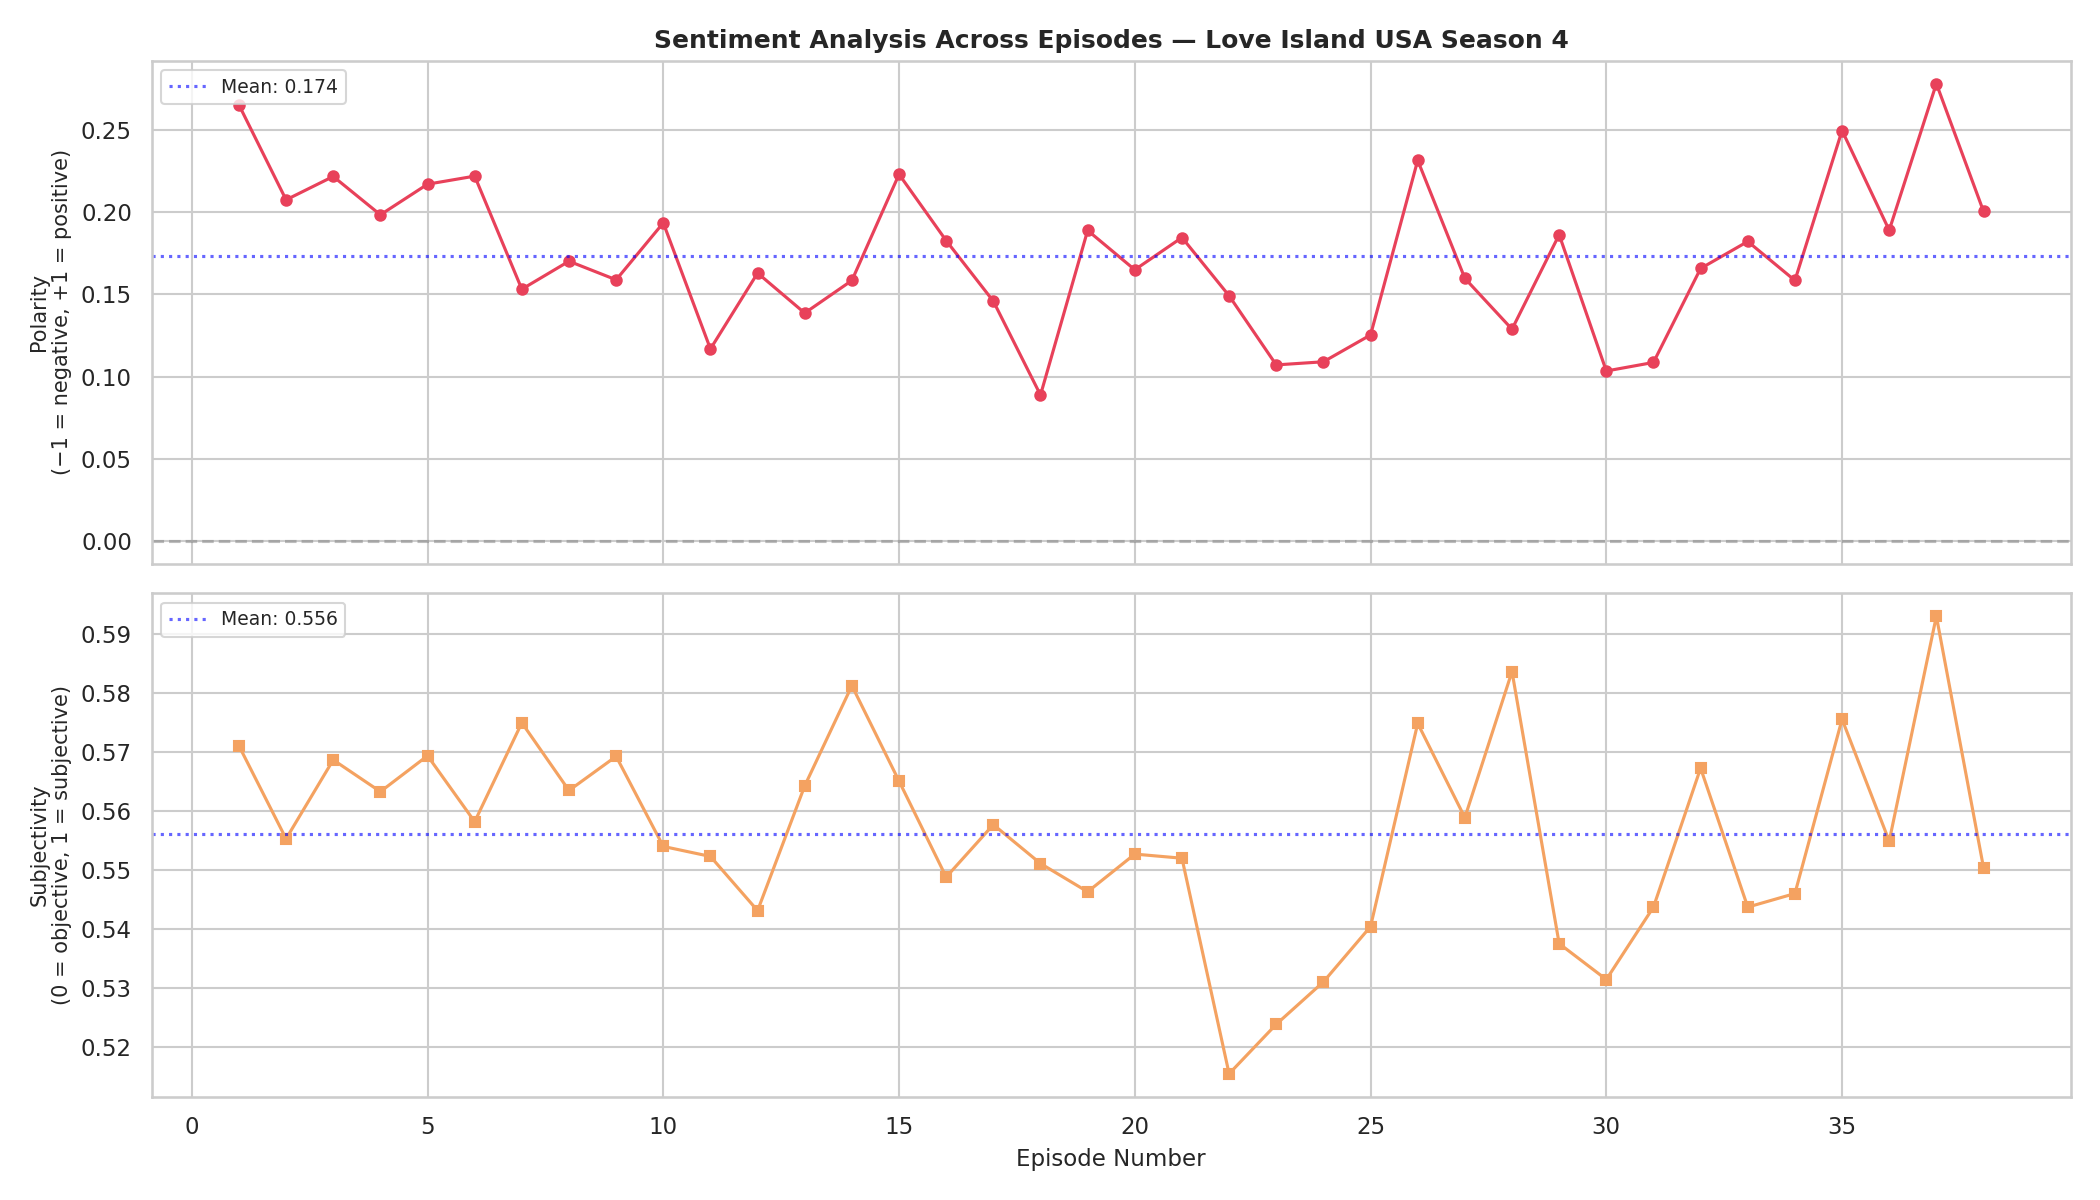
\includegraphics[width=0.82\linewidth,height=0.42\textheight,keepaspectratio]{08_sentiment_per_episode.png}
\caption*{\textbf{Figure 8.} Sentiment across episodes.}
\end{figure}

Removing function words, the most frequent content words are \emph{feel, love, good, think, want, going,} and \emph{get} (Figure 9) --- an emotion- and intention-focused vocabulary that fits the show's theme of romantic connection.

\begin{figure}[H]
\centering
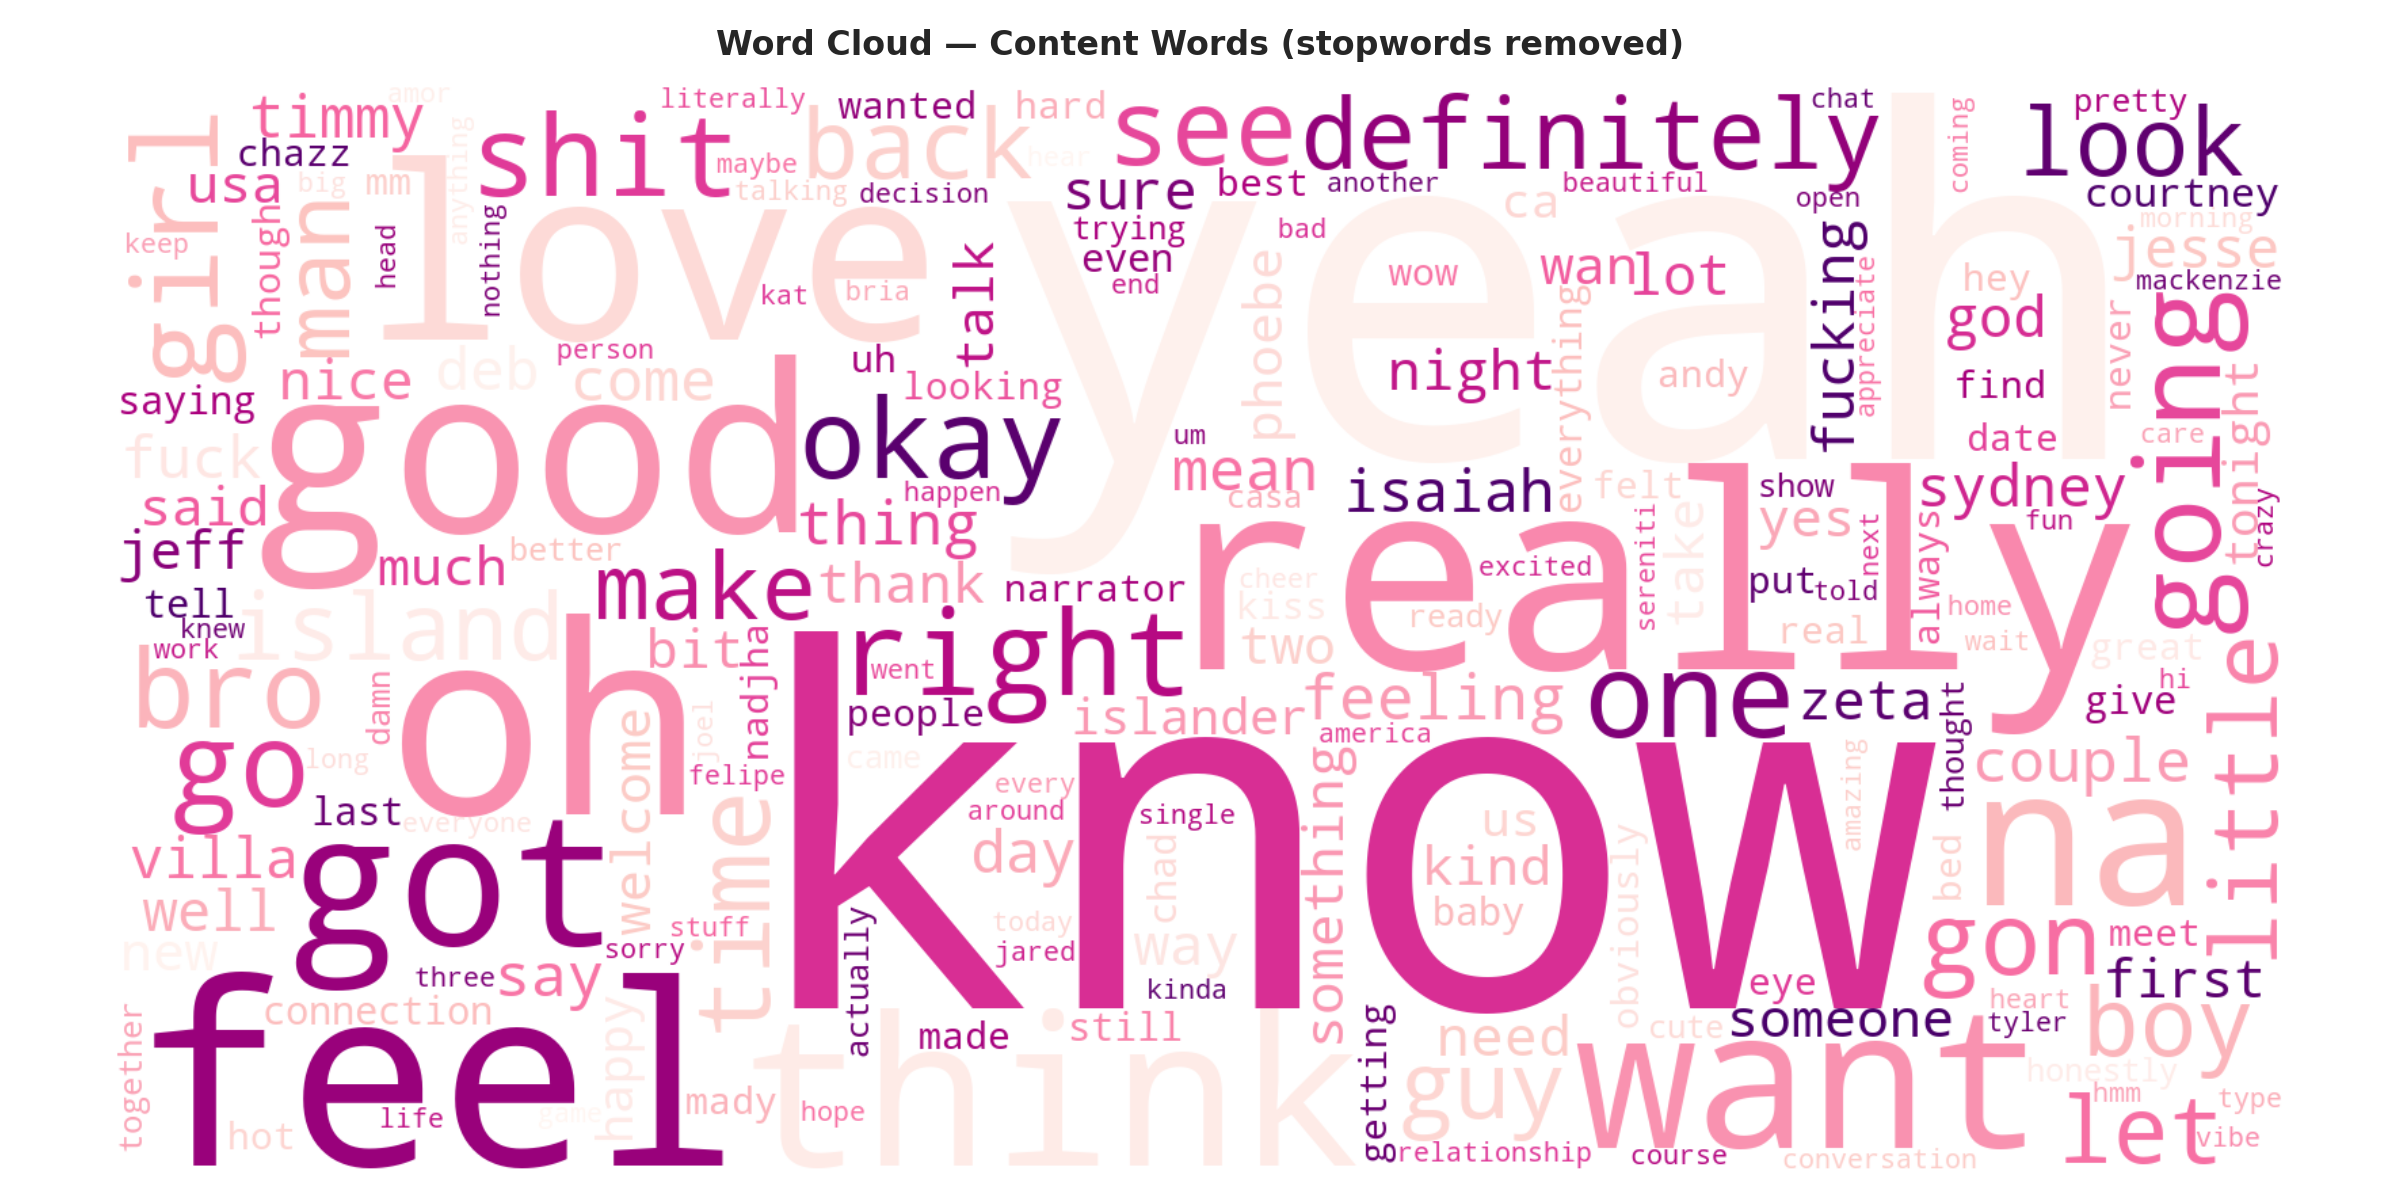
\includegraphics[width=0.82\linewidth,height=0.42\textheight,keepaspectratio]{05_wordcloud_no_stopwords.png}
\caption*{\textbf{Figure 9.} Word cloud of content words (function words removed).}
\end{figure}

\subsection*{4.8 Vocabulary growth across the season}

A related way to see the show's small vocabulary is to track how quickly \emph{new} words appear. Figure 10 plots cumulative unique word types against the running token count: the curve climbs steeply and then flattens, the signature of vocabulary saturation. About two-thirds (67.8\%) of the season's 7,856 word types have already appeared by the halfway point (end of Episode 19); later episodes mostly recombine an already-settled lexicon rather than introduce new vocabulary.

\begin{figure}[H]
\centering
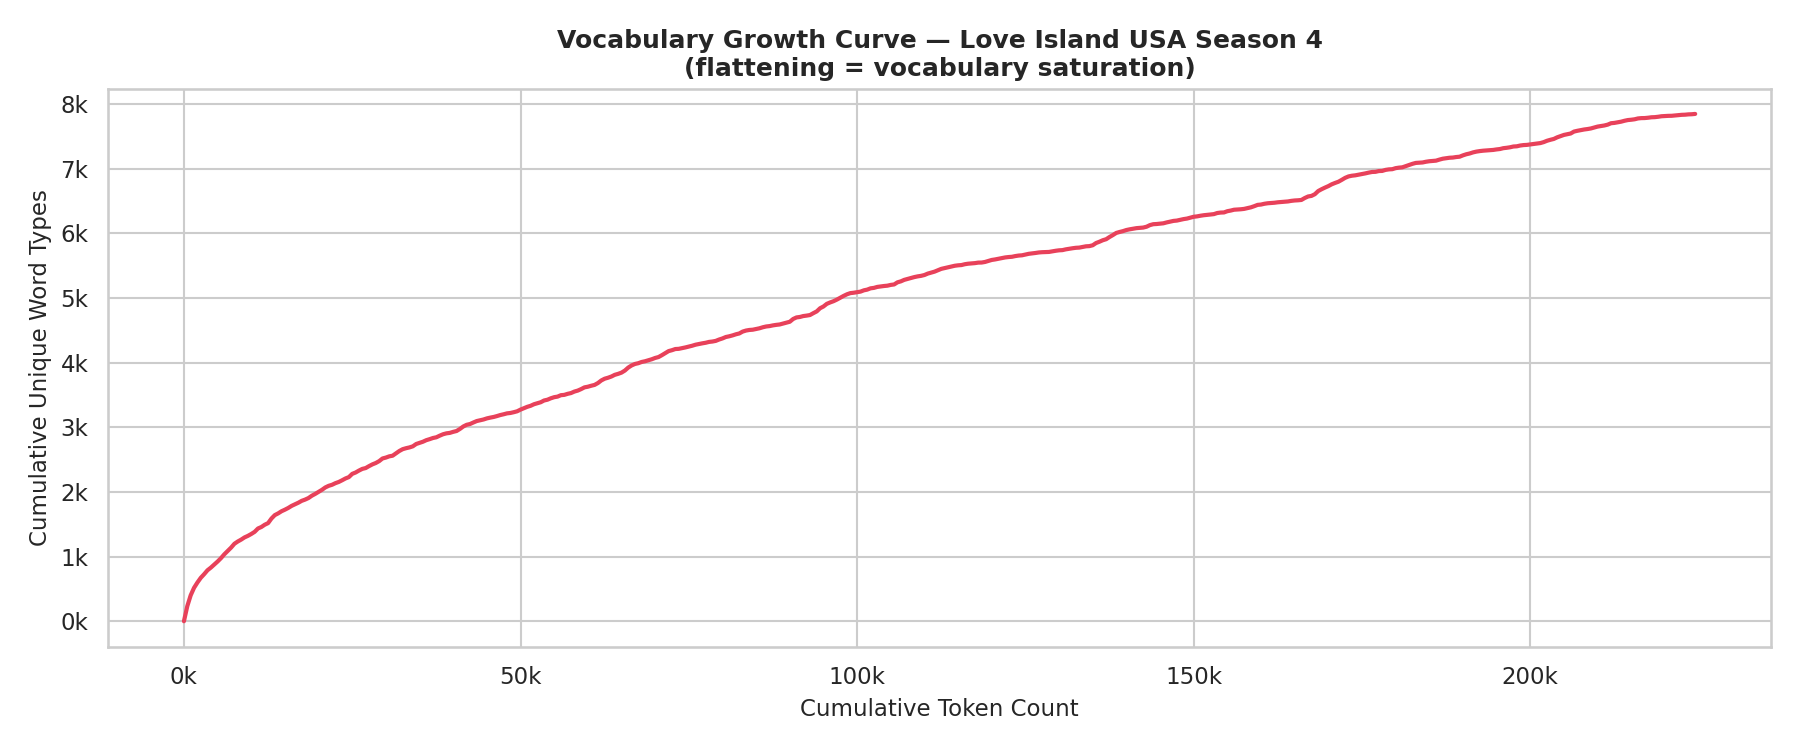
\includegraphics[width=0.82\linewidth,height=0.42\textheight,keepaspectratio]{10_vocabulary_growth_curve.png}
\caption*{\textbf{Figure 10.} Vocabulary growth curve.}
\end{figure}


\section*{5. Discussion}

Every measure points the same way: \emph{Love Island USA} Season 4 runs on a small, familiar, repeated vocabulary. The headline numbers for a general reader are the two new ones. \textbf{You can follow 95\% of the show on about 1,250 word families} --- well under the $\sim$3,000 needed for everyday English --- and the dialogue reads at roughly a \textbf{third- to fifth-grade level}, with 98\% of its words among the most familiar in English. This is a genuinely low-demand form of English.

That is unsurprising for spontaneous speech, which is always more restricted than writing, but the \emph{degree} is striking, and the near-perfect Zipfian fit (R\textsuperscript{2} = 0.98) shows the pattern is highly regular rather than a quirk of a few episodes. The texture of the talk explains the simplicity: it is emotional and personal (uniformly positive, highly subjective) but expressed through verbs, pronouns, intensifiers (\emph{really}, \emph{so}), and a thin band of evaluative adjectives (\emph{good}, \emph{amazing}, \emph{crazy}) rather than descriptive variety. Discourse markers like \emph{like} and \emph{know} form a structural layer that organises talk and signals informality more than it adds content. This matches Biber et al.'s (1999) "involved production" --- language under real-time pressure that foregrounds stance and connection over elaboration.

The implications cut two ways. For accessibility, the show is easy: learners of English, younger viewers, and the broad public can follow it almost completely, which is part of its mass appeal. For language exposure, that same narrowness means heavy viewing offers a repetitive linguistic diet --- a useful point for anyone weighing such content as "language input." A natural next step is a controlled comparison with scripted television of similar theme to isolate how much scripting widens vocabulary.


\section*{6. Limitations}

\begin{itemize}
\item \textbf{No speaker labels.} The subtitles mix contestant, host, and voiceover speech and many different contestants, so results describe the broadcast as a whole, not individuals. Speaker-diarised transcripts would be needed for person-level analysis.
\item \textbf{Approximations.} "Word families" were approximated by automatic lemmatisation, and reading-level/POS/sentiment tools are imperfect on informal, punctuation-stripped speech; figures are best read as robust \emph{relative} indicators rather than exact values. Readability formulas in particular disagree on the exact grade ($\approx$3 to $\approx$7), though all place the show low.
\item \textbf{Transcription quirks.} Captions can mis-hear names and slang, and contractions such as \emph{gonna} split into fragments (\emph{gon}/\emph{na}); single-letter words (\emph{I}, \emph{a}) were removed in preprocessing.
\item \textbf{Spread, not depth.} Coverage and diversity measure how \emph{many} words appear, not how precisely or creatively they are used.
\end{itemize}


\section*{7. Conclusion}

\emph{Love Island USA} Season 4 is, linguistically, a small and welcoming world. Across 224,815 words we find a tiny high-frequency core (top 100 words = 61\% of speech), low lexical diversity (MTLD 59.96), and a strongly positive, subjective tone carried by verbs rather than description. Most concretely: a viewer needs only about \textbf{1,250 common word families to understand 95\%} of the show, and the dialogue sits at roughly a \textbf{third- to fifth-grade reading level}, with 98\% of its words among the 3,000 most familiar in English. Whether that reflects the nature of unscripted emotional speech, the cast, or the demands of being on camera is a question for future work --- but the language of the villa, for all its drama, asks very little of its audience.


\FloatBarrier
\section*{References}

Adolphs, S., \& Schmitt, N. (2003). Lexical coverage of spoken discourse. \emph{Applied Linguistics, 24}(4), 425--438.

Biber, D., Johansson, S., Leech, G., Conrad, S., \& Finegan, E. (1999). \emph{Longman grammar of spoken and written English}. Pearson.

Channell, J. (1994). \emph{Vague language}. Oxford University Press.

Dale, E., \& Chall, J. S. (1948). A formula for predicting readability. \emph{Educational Research Bulletin, 27}(1), 11--28.

Fleiss, R. (2018). Vague language in reality television: Hedging as social performance. \emph{Journal of Sociolinguistics, 22}(3), 301--324.

Kincaid, J. P., Fishburne, R. P., Rogers, R. L., \& Chissom, B. S. (1975). \emph{Derivation of new readability formulas for Navy enlisted personnel}. Naval Technical Training Command.

McCarthy, P. M., \& Jarvis, S. (2010). MTLD, vocd-D, and HD-D: A validation study of sophisticated approaches to lexical diversity assessment. \emph{Behavior Research Methods, 42}(2), 381--392.

Nation, I. S. P. (2001). \emph{Learning vocabulary in another language}. Cambridge University Press.

Nation, I. S. P. (2006). How large a vocabulary is needed for reading and listening? \emph{Canadian Modern Language Review, 63}(1), 59--82.

Richards, B. (1987). Type/token ratios: What do they really tell us? \emph{Journal of Child Language, 14}(2), 201--209.

Thornborrow, J., \& Morris, D. (2004). Gossip as strategy: The management of talk about others on reality TV show \emph{Big Brother}. \emph{Journal of Sociolinguistics, 8}(2), 246--271.

Webb, S., \& Rodgers, M. P. H. (2009). The vocabulary demands of television programs. \emph{Language Learning, 59}(2), 335--366.


\FloatBarrier
\needspace{0.18\textheight}
\section*{Appendix A --- Vocabulary Load and Reading Level}

\emph{Vocabulary load: word families needed for each coverage level (lemmatised); raw word types shown for comparison.}

\begin{center}
\begin{tabular}{lll}
\toprule
Coverage of show & Word families needed & Raw word types needed \\
\midrule
80\% & 250 & 326 \\
90\% & 592 & 860 \\
95\% & 1,249 & 1,902 \\
98\% & 2,554 & 3,911 \\
\bottomrule
\end{tabular}
\end{center}

\emph{Benchmark for everyday/spoken English: $\sim$3,000 families for 95\%, $\sim$6,000--7,000 for 98\% (Adolphs \& Schmitt, 2003; Nation, 2006; Webb \& Rodgers, 2009).}

\emph{Reading level of the full corpus:}

\begin{center}
\begin{tabular}{p{0.431\linewidth}lp{0.419\linewidth}}
\toprule
Measure & Value & Interpretation \\
\midrule
Flesch--Kincaid Grade & 2.8 & $\sim$3rd grade \\
Consensus grade (textstat) & 3.0 & $\sim$3rd grade \\
Flesch Reading Ease & 90.2 & "very easy" (90--100) \\
SMOG Index & 6.9 & $\sim$7th grade (syllable-weighted) \\
\% words outside 3,000 familiar list & 2.1\% & 97.9\% of words are highly familiar \\
Per-episode FK grade range & 2.3--3.7 & consistently easy \\
\bottomrule
\end{tabular}
\end{center}

\FloatBarrier
\needspace{0.46\textheight}
\section*{Appendix B --- Corpus Statistics by Episode}

\emph{Tokens = post-cleaning token count; Types = unique word types.}

\begin{center}
\small\setlength{\tabcolsep}{4pt}
\begin{tabular}{lllllllllll}
\toprule
Ep & Tokens & Types & TTR & MTLD &  & Ep & Tokens & Types & TTR & MTLD \\
\midrule
1 & 8650 & 1273 & 0.147 & 59.21 &  & 20 & 5973 & 1076 & 0.180 & 60.86 \\
2 & 7062 & 1108 & 0.157 & 43.24 &  & 21 & 6031 & 961 & 0.159 & 59.93 \\
3 & 5930 & 995 & 0.168 & 61.90 &  & 22 & 8294 & 1130 & 0.136 & 55.45 \\
4 & 5722 & 936 & 0.164 & 53.98 &  & 23 & 5656 & 910 & 0.161 & 64.50 \\
5 & 5415 & 1158 & 0.214 & 81.93 &  & 24 & 6174 & 1227 & 0.199 & 60.16 \\
6 & 5317 & 920 & 0.173 & 62.15 &  & 25 & 5171 & 947 & 0.183 & 58.74 \\
7 & 5447 & 953 & 0.175 & 59.85 &  & 26 & 5617 & 979 & 0.174 & 64.88 \\
8 & 6468 & 950 & 0.147 & 56.49 &  & 27 & 6337 & 1032 & 0.163 & 53.28 \\
9 & 5038 & 956 & 0.190 & 67.12 &  & 28 & 4675 & 896 & 0.192 & 67.98 \\
10 & 6087 & 1009 & 0.166 & 55.08 &  & 29 & 4883 & 909 & 0.186 & 56.19 \\
11 & 5961 & 1259 & 0.211 & 62.39 &  & 30 & 5244 & 1286 & 0.245 & 55.98 \\
12 & 5009 & 998 & 0.199 & 65.01 &  & 31 & 5959 & 970 & 0.163 & 55.62 \\
13 & 5411 & 887 & 0.164 & 54.69 &  & 32 & 5167 & 983 & 0.190 & 61.26 \\
14 & 4750 & 918 & 0.193 & 63.41 &  & 33 & 4790 & 920 & 0.192 & 54.69 \\
15 & 5368 & 922 & 0.172 & 51.89 &  & 34 & 4763 & 923 & 0.194 & 61.50 \\
16 & 5275 & 997 & 0.189 & 54.35 &  & 35 & 7932 & 1044 & 0.132 & 43.82 \\
17 & 5407 & 1276 & 0.236 & 64.92 &  & 36 & 6007 & 1240 & 0.206 & 40.42 \\
18 & 5249 & 910 & 0.173 & 76.77 &  & 37 & 6034 & 1068 & 0.177 & 67.58 \\
19 & 5176 & 996 & 0.192 & 71.49 &  & 38 & 11366 & 1415 & 0.125 & 69.80 \\
\bottomrule
\end{tabular}
\end{center}

\FloatBarrier
\needspace{0.9\textheight}
\section*{Appendix C --- Top 100 Words}

\emph{Single-character tokens (e.g., I, a) excluded by preprocessing. Note the appearance of contestant first names (Isaiah, Timmy, Sydney, Deb), informal markers (bro), and tokeniser fragments of contractions (na ← gonna/wanna, gon ← gonna) within the high-frequency band.}

\begin{center}
\footnotesize\setlength{\tabcolsep}{4pt}
\begin{tabular}{llllllll}
\toprule
Rank & Word & Count & \% & Rank & Word & Count & \% \\
\midrule
1 & you & 9228 & 4.105 & 51 & did & 815 & 0.363 \\
2 & to & 6545 & 2.911 & 52 & go & 814 & 0.362 \\
3 & like & 6338 & 2.819 & 53 & at & 809 & 0.36 \\
4 & the & 5972 & 2.656 & 54 & get & 806 & 0.359 \\
5 & and & 5289 & 2.353 & 55 & they & 805 & 0.358 \\
6 & it & 4684 & 2.083 & 56 & her & 803 & 0.357 \\
7 & that & 4592 & 2.043 & 57 & one & 793 & 0.353 \\
8 & know & 2920 & 1.299 & 58 & out & 751 & 0.334 \\
9 & yeah & 2802 & 1.246 & 59 & shit & 731 & 0.325 \\
10 & do & 2702 & 1.202 & 60 & okay & 715 & 0.318 \\
11 & just & 2604 & 1.158 & 61 & now & 702 & 0.312 \\
12 & is & 2595 & 1.154 & 62 & if & 693 & 0.308 \\
13 & so & 2408 & 1.071 & 63 & would & 690 & 0.307 \\
14 & in & 2299 & 1.023 & 64 & can & 680 & 0.302 \\
15 & of & 2244 & 0.998 & 65 & bro & 674 & 0.3 \\
16 & me & 2182 & 0.971 & 66 & him & 633 & 0.282 \\
17 & was & 2100 & 0.934 & 67 & see & 625 & 0.278 \\
18 & for & 2083 & 0.927 & 68 & gon & 595 & 0.265 \\
19 & with & 2061 & 0.917 & 69 & definitely & 570 & 0.254 \\
20 & we & 2036 & 0.906 & 70 & time & 565 & 0.251 \\
21 & what & 1978 & 0.88 & 71 & because & 563 & 0.25 \\
22 & my & 1962 & 0.873 & 72 & back & 557 & 0.248 \\
23 & this & 1570 & 0.698 & 73 & island & 515 & 0.229 \\
24 & have & 1556 & 0.692 & 74 & been & 509 & 0.226 \\
25 & be & 1510 & 0.672 & 75 & let & 502 & 0.223 \\
26 & on & 1505 & 0.669 & 76 & girl & 501 & 0.223 \\
27 & he & 1482 & 0.659 & 77 & who & 498 & 0.222 \\
28 & really & 1456 & 0.648 & 78 & man & 493 & 0.219 \\
29 & but & 1404 & 0.625 & 79 & little & 486 & 0.216 \\
30 & oh & 1382 & 0.615 & 80 & more & 478 & 0.213 \\
31 & are & 1369 & 0.609 & 81 & as & 461 & 0.205 \\
32 & up & 1210 & 0.538 & 82 & from & 444 & 0.197 \\
33 & all & 1194 & 0.531 & 83 & when & 440 & 0.196 \\
34 & feel & 1174 & 0.522 & 84 & had & 434 & 0.193 \\
35 & love & 1137 & 0.506 & 85 & look & 432 & 0.192 \\
36 & not & 1128 & 0.502 & 86 & say & 431 & 0.192 \\
37 & she & 1101 & 0.49 & 87 & or & 430 & 0.191 \\
38 & good & 1079 & 0.48 & 88 & isaiah & 427 & 0.19 \\
39 & think & 1035 & 0.46 & 89 & timmy & 424 & 0.189 \\
40 & about & 938 & 0.417 & 90 & very & 417 & 0.185 \\
41 & how & 938 & 0.417 & 91 & mean & 416 & 0.185 \\
42 & your & 924 & 0.411 & 92 & too & 408 & 0.181 \\
43 & na & 906 & 0.403 & 93 & come & 401 & 0.178 \\
44 & there & 906 & 0.403 & 94 & fuck & 398 & 0.177 \\
45 & want & 851 & 0.379 & 95 & sydney & 397 & 0.177 \\
46 & here & 842 & 0.375 & 96 & deb & 396 & 0.176 \\
47 & got & 837 & 0.372 & 97 & fucking & 387 & 0.172 \\
48 & going & 818 & 0.364 & 98 & will & 386 & 0.172 \\
49 & right & 817 & 0.363 & 99 & well & 382 & 0.17 \\
50 & no & 815 & 0.363 & 100 & make & 381 & 0.169 \\
\bottomrule
\end{tabular}
\end{center}

\FloatBarrier
\needspace{0.46\textheight}
\section*{Appendix D --- Sentiment Scores by Episode}

\emph{TextBlob polarity ($-$1 to +1) and subjectivity (0 to 1), computed over full episode text.}

\begin{center}
\small\setlength{\tabcolsep}{4pt}
\begin{tabular}{llllll}
\toprule
Ep & Polarity & Subjectivity & Ep & Polarity & Subjectivity \\
\midrule
1 & 0.2651 & 0.5711 & 20 & 0.1649 & 0.5527 \\
2 & 0.2074 & 0.5553 & 21 & 0.1845 & 0.552 \\
3 & 0.2216 & 0.5687 & 22 & 0.1491 & 0.5154 \\
4 & 0.1983 & 0.5633 & 23 & 0.1071 & 0.5238 \\
5 & 0.2169 & 0.5694 & 24 & 0.109 & 0.531 \\
6 & 0.2218 & 0.5582 & 25 & 0.1253 & 0.5404 \\
7 & 0.1531 & 0.575 & 26 & 0.2314 & 0.5749 \\
8 & 0.1701 & 0.5635 & 27 & 0.1597 & 0.5589 \\
9 & 0.1588 & 0.5693 & 28 & 0.1288 & 0.5837 \\
10 & 0.1934 & 0.554 & 29 & 0.1862 & 0.5375 \\
11 & 0.1168 & 0.5523 & 30 & 0.1034 & 0.5314 \\
12 & 0.1629 & 0.5431 & 31 & 0.1086 & 0.5437 \\
13 & 0.1386 & 0.5643 & 32 & 0.1657 & 0.5673 \\
14 & 0.1584 & 0.5813 & 33 & 0.1821 & 0.5437 \\
15 & 0.2229 & 0.5651 & 34 & 0.1584 & 0.546 \\
16 & 0.1826 & 0.5488 & 35 & 0.2495 & 0.5756 \\
17 & 0.1458 & 0.5577 & 36 & 0.1889 & 0.5549 \\
18 & 0.0888 & 0.5511 & 37 & 0.278 & 0.5931 \\
19 & 0.1888 & 0.5463 & 38 & 0.2004 & 0.5504 \\
\bottomrule
\end{tabular}
\end{center}

\FloatBarrier
\needspace{0.27\textheight}
\section*{Appendix E --- Statistical Tests}

\emph{Trend correlations are across the 38 episodes (n = 38); Zipf regression is over all ranked word types. Full filler-word counts available on request.}

\begin{center}
\begin{tabular}{p{0.534\linewidth}p{0.316\linewidth}l}
\toprule
Test & Statistic & p-value \\
\midrule
Top 10 / 50 / 100 / 1,000 words --- \% of all tokens & 22.7\% / 48.7\% / 61.0\% / 91.1\% & --- \\
Zipf regression slope (log freq $\sim$ log rank) & $-$1.453 & $<$ .001 \\
Zipf regression R\textsuperscript{2} & 0.981 & --- \\
MTLD vs. episode --- Pearson r & $-$0.107 & .521 \\
MTLD vs. episode --- Spearman $\rho$ & $-$0.028 & .868 \\
TTR vs. episode --- Pearson r & 0.048 & .775 \\
TTR vs. episode --- Spearman $\rho$ & 0.109 & .514 \\
Sentiment polarity vs. episode --- Pearson r & $-$0.129 & .441 \\
Sentiment polarity vs. episode --- Spearman $\rho$ & $-$0.149 & .371 \\
\bottomrule
\end{tabular}
\end{center}


\emph{Analysis performed using Python 3.12. Scripts (\texttt{analyze\_love\_island.py}, \texttt{analyze\_vocab\_level.py}), the cleaned corpus, and all output tables/figures are available on request.}

\end{document}
